\documentclass[tikz,border=10pt]{standalone}
\begin{document}
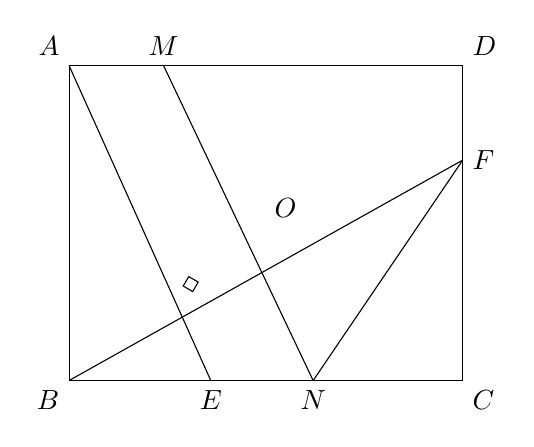
\begin{tikzpicture}[scale=1]

\coordinate (A) at (0,4);
\coordinate (B) at (0,0);
\coordinate (C) at (5,0);
\coordinate (D) at (5,4);
\coordinate (M) at (1.2,4);
\coordinate (E) at (1.8,0);
\coordinate (N) at (3.1,0);
\coordinate (F) at (5,2.8);
\coordinate (O) at (2.75,1.95);

\draw (A) -- (B) -- (C) -- (D) -- cycle;
\draw (A) -- (E);
\draw (M) -- (N);
\draw (B) -- (F);
\draw (N) -- (F);

\draw (1.45,1.2) -- (1.57,1.13) -- (1.64,1.25) -- (1.52,1.32) -- cycle;

\node[above left] at (A) {$A$};
\node[below left] at (B) {$B$};
\node[below right] at (C) {$C$};
\node[above right] at (D) {$D$};
\node[above] at (M) {$M$};
\node[below] at (E) {$E$};
\node[below] at (N) {$N$};
\node[right] at (F) {$F$};
\node[above] at (O) {$O$};

\end{tikzpicture}
\end{document}
